\documentclass[12pt,a4paper]{report}
\usepackage[italian]{babel}
\usepackage{newlfont}
\usepackage{color}
\textwidth=450pt\oddsidemargin=0pt

\usepackage[utf8x]{inputenc}
\usepackage{graphicx}
\usepackage{amsmath}
\usepackage{amssymb}
\usepackage{setspace}

\begin{document}

% qui comincia il titolo
\begin{titlepage}
\begin{center}
{\Large{\textsc{Università degli studi di Roma $\cdot$ Tor Vergata}}}
\rule[0.1cm]{15.8cm}{0.1mm}
\rule[0.5cm]{15.8cm}{0.6mm}
\\\vspace{3mm}

{\small{\bf Macroarea di Lettere e Filosofia \\ Master in Sonic Arts}}

\end{center}

\vspace{23mm}

\begin{center}
\begin{spacing}{1.7}
\textcolor{black}{
\linespread{5}
{\LARGE{\bf
Audio Object-Oriented e adattamento del formato Multi-Dimensional Audio MDA alle configurazioni 2.0, 5.1 e 4.0 attraverso la tecnica di spazializzazione Vector-Base Amplitude Panning VBAP.
}}}

\end{spacing}
\end{center}

\vspace{50mm} \par \noindent

\begin{minipage}[t]{0.47\textwidth}

{\large{\bf Relatore: \vspace{2mm}\\\textcolor{black}{
Prof. Giuseppe Silvi}\\\\

%\textcolor{red}{
%\bf Correlatore: (eventuale)
%\vspace{2mm}\\
%Prof./Dott . Nome Cognome\\\\}
}
}
\end{minipage}
%
\hfill
%
\begin{minipage}[t]{0.47\textwidth}\raggedleft \textcolor{black}{
{\large{\bf Presentata da:
\vspace{2mm}\\
Lorenzo Ferri}}}
\end{minipage}

\vspace{5mm}

\begin{center}

{\large{%\bf Sessione \textcolor{black}{ I }
%\vspace{2mm}\\

Anno Accademico \textcolor{black}{2016/17}}}
\end{center}

\newpage\null\thispagestyle{empty}

\end{titlepage}
% qui finisce il titolo

\tableofcontents

\listoffigures


\addcontentsline{toc}{chapter}{Elenco delle figure}

\chapter*{Abstract}

L'obbiettivo di questa tesi è quello di implementare un algoritmo che permetta di riprodurre un contenuto sonoro orientato agli oggetti su una configurazione di riproduzione facilmente riscontrabile in un ambiente domestico.

In un primo momento, infatti, andrò a spiegare che cosa sono le configurazioni multicanale $2.0, 4.0$ e $5.1$ inoltre introdurrò l'audio object-oriented con particolare riguardo al formato ad oggetti Multi-Dimensional Audio MDA, in un secondo momento invece cercherò di implementare l'MDA nelle configurazioni multicanale descritte servendomi della tecnica di spazializzazione \textbf{Vector-Base Amplitude Panning VBAP} di cui spiegherò anche il funzionamento.

Infine farò degli esempi.

\addcontentsline{toc}{chapter}{Abstract}

\chapter{Dai canali audio agli oggetti sonori}

Premetto che in questo testo non affronterò tutti gli aspetti della produzione sonora e dell'ascolto, toccherò invece solo quegli aspetti che riguardano la collocazione spaziale degli oggetti sonori\footnote{Con oggetto sonoro intendo quell'entità che contiene l'informazione sonora registrata da un microfono o creata virtualmente che viene elaborata in fase di produzione singolarmente} trattando, quindi, le configurazioni spaziali dei diffusori in fase di produzione in studio e di ascolto a casa.

Nel mondo odierno l'avanzamento tecnologico ha permesso a tutti coloro che ne hanno voglia la possibilità di poter ascoltare un contenuto sonoro in ambiente domestico in modo semplice, basti pensare a chi ascolta un disco musicale in un impianto hi-fi o a chi invece gode dell'ascolto surround\footnote{Con surround si intende quel tipo di ascolto in cui l'ascoltatore è immerso nella scena sonora, per fare questo tipicamente si collocano diffusori ai lati e/o dietro l'ascoltatore} di un film in un impianto home-theater, in tutti questi casi la persona interessata possiede un prodotto sonoro che viene ascoltato attraverso l'impianto audio posseduto in casa, questo è possibile grazie ad una complessa catena di produzione e di ascolto sonoro che da la possibilità a tutti di poter ascoltare il contenuto esattamente come è stato creato.

Quello che sta alla base di tutta questa catena è il produttore, esso per riuscire a creare al meglio il contenuto e per dare la giusta collocazione spaziale agli oggetti sonori deve essere a conoscenza del modo in cui l'ascoltatore ascolta il suo prodotto, infatti esso adotterà un metodo di lavoro che prevede l'allestimento di un impianto audio in studio con le stesse specifiche spaziali (posizione e numero di diffusori) di quello che normalmente adotterebbe l'ascoltatore in casa per l'ascolto di quel contenuto, adottando questa soluzione è sicuro di creare un prodotto che ha la giusta collocazione spaziale di ogni oggetto sonoro e che l'ascoltatore senta la medesima cosa.

Successivamente, il produttore riverserà il contenuto sonoro codificato in certo formato\footnote{Con formato audio intendo il protocollo e le specifiche con cui è creato e memorizzato un contenuto sonoro all'interno di un supporto} all'interno di un supporto che verrà poi acquistato dall'ascoltatore e riprodotto in casa dal suo impianto, logicamente l'impianto deve avere un lettore in grado di poter supportare il formato e in grado (attraverso specifiche decodifiche) di associare a ogni diffusore un canale audio da riprodurre.

Per fare un esempio consideriamo l'ascolto di un disco in un impianto hi-fi, nella maggior parte dei casi in cui della musica sia creata in studio di registrazione si opera in modo che per tutta la sua produzione si rispetti un certo standard nella collocazione dei monitor all'interno dello studio, stessa cosa dovrebbe fare l'ascoltatore a casa per usufruire della stessa informazione musicale, infatti in questo caso sia i fonici che l'ascoltatore dovrebbero rispettare lo standard dato dalla configurazione 2.0 contenuta nella specifica \cite{5.1} per rientrare nel modo più comune di produzione ed ascolto di contenuti puramente musicali.

Stesso discorso si può fare per l'ascolto surround di contenuti sonori di un film solo che in questo caso, sia in studio che a casa, si a avrà una configurazione adatta rispettivamente alla creazione e alla riproduzione di un suono surround tipico di una pellicola cinematografica, una configurazione possibile e che è la maggiore impiegata in ambito domestico è la 5.1 data anch'essa dalla specifica \cite{5.1}.

In tutti due i casi il produttore e l'ascoltatore seguono lo stesso standard di collocazione spaziale dei diffusori , quindi di conseguenza quest'ultimo ascolterà esattamente quello che il produttore vuole che si senta (si parlerà sempre di collocazione degli oggetti sonori); spesso però capita che l'ascoltatore non è in possesso un impianto in grado di riprodurre spazialmente il contenuto di un prodotto sonoro (per esempio basti pensare a chi vuole sentire un audio surround di un film in un comune hi-fi) e che quindi non in grado di rispettare lo standard della catena sopra proposta.

In questi casi esistono degli algoritmi che a patto di sacrificare la corretta ricostruzione dell'ambiente sonoro, riescono a far riprodurre in un impianto configurato spazialmente in una certa maniera un prodotto musicale non destinato nativamente ad esso.

Ora, prima di trattare un esempio di uno di questi algoritmi, è d'obbligo fermarsi un attimo e percorrere brevemente quali sono le specifiche degli standard appena citati e introdurre la configurazione $4.0$ che tratterò in questa tesi.

\section{Configurazioni di riproduzione 2.0, 5.1 e 4.0}\label{metodi}

Nell'audio, quando si parla di configurazione spaziale, è norma usare un codice numerico standard che sta ad indicare sinteticamente il numero di diffusori sonori usati e la loro funzione, questo codice è composto da tre numeri separati da punti nel formato $X.Y.Z$ dove $X$ sta ad indicare il numero di diffusori disposti orizzontalmente sul piano attorno l'ascoltatore, $Y$ sta ad indicare il numero di diffusori imputati alla riproduzione del canale LFE\footnote{l'LFE (acronimo di Low Frequency Effect) è quel canale imputato alla riproduzione degli effetti a bassa frequenza tipicamente riprodotti da uno o più subwoofer} e $Z$ sta per il numero di diffusori posti sopra l'ascoltatore per ampliare l'ascolto anche verticalmente.

La prima configurazione descritta è la \textbf{2.0} che come da specifica ITU-R BS.775-3\cite{5.1} prevede l'utilizzo di due diffusori (di norma full-range\footnote{In realtà si potrebbe usare anche un subwoofer in aiuto ai due diffusori per quanto riguarda la zona frequenziale bassa}) posti di fronte all'ascoltatore e con angoli di $\pm 30°$ come in figura \ref{fig:2.0}

Tipicamente la sensazione di collocazione spaziale di una sorgente sonora in questa configurazione viene data dalla differenza di potenza del segnale inviato ai due speaker, infatti se il segnale risulta più forte in uno dei due, la sorgente fantasma risulterà più spostata verso quest'ultimo in accordo con le argomentazioni scritte in \cite{vbap}.

E' consuetudine indicare rispettivamente con L (left) ed R (right) lo speaker posto di fronte a sinistra e a destra dell'ascoltatore.

\begin{figure}[htbp]
	\centering
	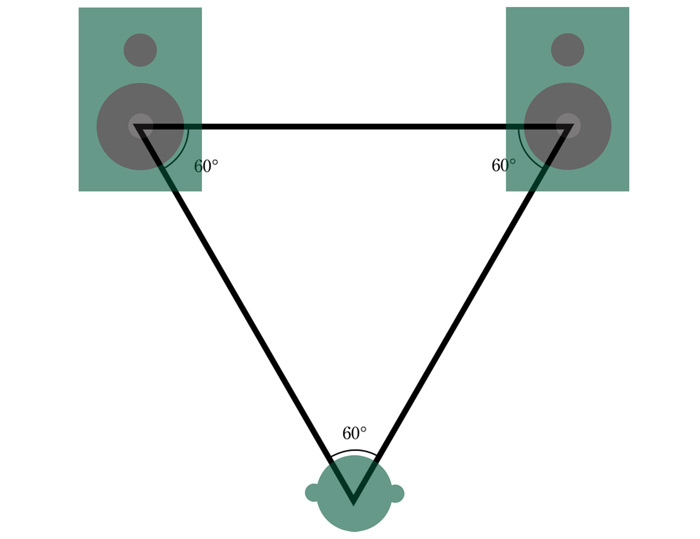
\includegraphics[scale=0.30]{figures/stereo.jpg}
	\caption {Configurazione 2.0 (ITU-R BS.775-3)}
	\label{fig:2.0}
	\end{figure}
	
Per quanto riguarda un ascolto surround, invece, ci si riferisce a un tipo di riproduzione che pone l'ascoltatore al centro di un piano di diffusione in modo che si possano sentire suoni provenienti anche dai lati e da dietro; diverse sono le configurazioni possibili ma quella che interessa a noi è la 5.1 data dalla specifica ITU-R BS 775-3\cite{5.1}.

Questa configurazione spaziale (quasi sicuramente la più diffusa in ambito surround domestico) è composta da 5 canali distribuiti in 5 diffusori disposti rispettivamente a $0°$, $\pm30°$ e $\pm110/120°$ e un canale LFE riprodotto da un subwoofer posto tipicamente davanti l'ascoltatore (In realtà il collocamento del subwoofer non è strettamente indicato nelle specifiche in quanto la natura delle basse frequenze le rende omnidirezionali, invece nelle specifiche è riportato il fatto che il canale LFE deve avere un incremento del segnale di $+10dB$.

In figura \ref{fig:5.1} possiamo vedere come sono disposti i 5 diffusori ma è da notare che non è riportata la posizione del subwoofer per il discorso appena affrontato.

E' norma indicare i diffusori come C (center) per il diffusore centrale, L (left) ed R (right) per i diffusori rispettivamente a $\pm30°$ (è consuetudine poi usare casse full-range per la coppia L-R), LS (left-surround) ed RS (right-surround) per i diffusori rispettivamente a $\pm110/120°$ .

\begin{figure}[htbp]
	\centering
	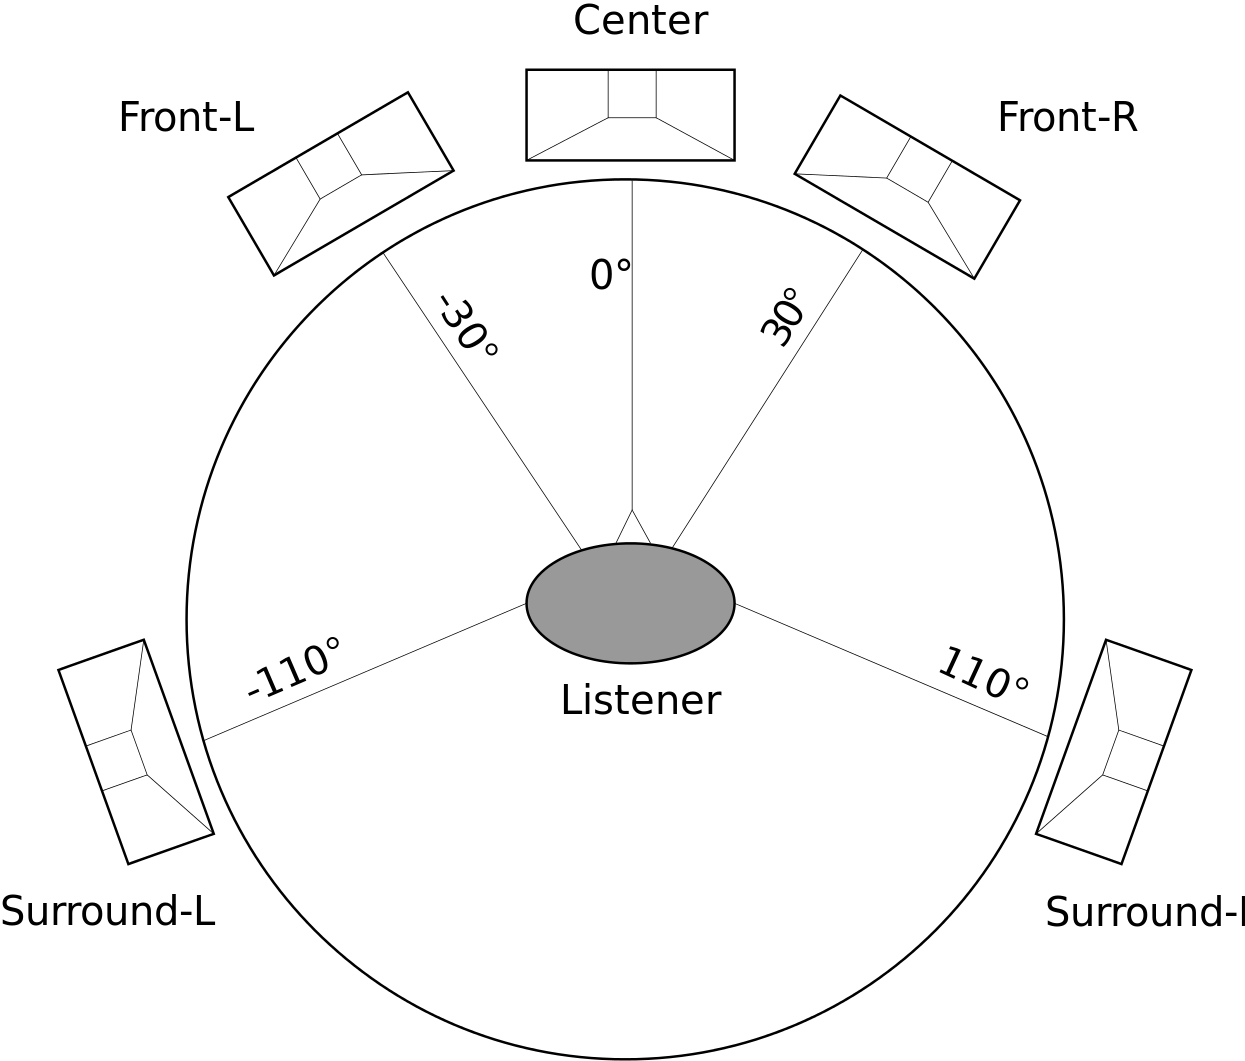
\includegraphics[scale=0.18]{figures/5-1.png}
	\caption {Configurazione 5.1 (ITU-R BS.775-3)}
	\label{fig:5.1}
	\end{figure}

In parallelo una configurazione che si potrebbe trovare in ambito domestico per la sua facilità di implementazione e la 4.0; questa tecnica prevede l'utilizzo di 4 speaker posti sui vertici di un quadrato (angoli di $\pm45°$ e $\pm135°$) con al centro l'ascoltatore.

Usualmente in letteratura si denominano la coppia di diffusori posti di fronte come LF (left-front) - RF (right-front) e la coppia posta dietro come LB (left-back) - RB (right-back), questi per riprodurre al meglio il contenuto sonoro dovrebbero essere full-range.

Per quanto riguarda questa configurazione c'è da dire che questo posizionamento crea dei problemi di percezione del contenuto spaziale in quanto il nostro udito è più sensibile a ciò che proviene di fronte a noi, questo costituisce un problema per i nostri scopi ma prenderemo lo stesso la configurazione in considerazione in quanto è possibile che in ambito domestico qualcuno possieda ancora un impianto 4.0 (anche se largamente in disuso).

\begin{figure}[htbp]
	\centering
	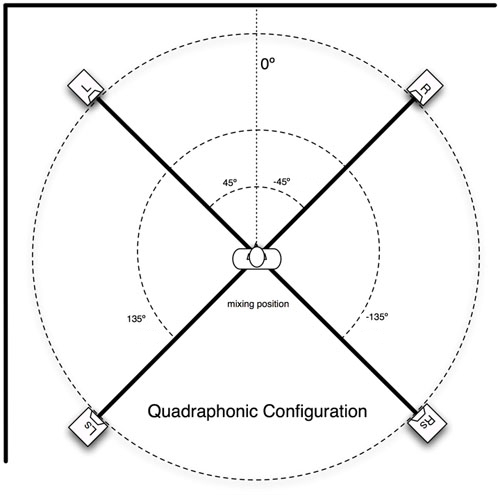
\includegraphics[scale=0.35]{figures/quad.jpg}
	\caption {Configurazione 4.0}
	\label{fig:quadrifonia}
	\end{figure}

\[\thicksim\blacklozenge \thicksim \]

Abbiamo visto quindi che lo stesso standard sulla collocazione spaziale dei diffusori di viene mantenuta dalla fase di produzione a quella di ascolto ma prima ho accennato del fatto che non è sempre così, infatti è possibile ascoltare in un impianto configurato secondo una certa specifica un contenuto sonoro non creato per esso con l'ausilio di algoritmi che permettono di rendere le configurazioni spaziali dei diffusori intercambiabili.

Per fare un esempio, la specifica ITU-R BS.775-3 definisce il modo in cui posso adattare un prodotto sonoro in una configurazione 2.0 ma che originariamente è stato creato per un 5.1.

l'algoritmo si basa sul fatto che la decodifica da una configurazione all'altra la ottengo combinando linearmente i canali della configurazione di partenza per ottenere quelli di arrivo, infatti nel testo è presente una matrice di decodifica dove in ingresso abbiamo 5 dei canali del 5.1 ed in uscita abbiamo i 2 canali del 2.0,infatti risulta che L' ed R' sono combinazione lineare di L, R, C, LS, RB secondo i coefficienti tabulati sotto.

\begin{figure}[htbp]
	\centering
	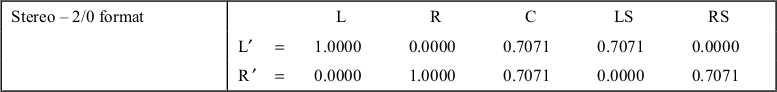
\includegraphics[scale=0.5]{figures/5-1to2-0.png}
	\caption {matrice di decodifica da 5.1 a 2.0}
	\label{fig:decodifica}
	\end{figure}

Per quanto riguarda il canale LFE esso va aumentato di $+10dB$ prima di ripartirlo nei due canali L ed R (ad ogni ripartizione poi va scalato di $-6dB$ per controbilanciare il raddoppio del segnale).

Abbiamo visto quindi un esempio di algoritmo che rende un contenuto sonoro adatto ad una riproduzione 5.1 intercambiabile con un 2.0.

\section{Formato audio object-oriented}

Ora capito quali sono i principali standard di riproduzione ci interessa capire il legame che c'è tra formato audio, canale audio e riproduzione in un impianto. 

Abbiamo detto in precedenza che il produttore riversa in un supporto il contenuto sonoro in certo formato, non ci interessano tanto le specifiche che stanno alla base di quest'ultimo ma ci interessa capire che ogni formato prevede al suo interno l'esistenza di un certo numero flussi di segnale, questi ultimi andranno a costituire, con o senza opportune codifiche, i canali audio per poter pilotare l'impianto, faccio un esempio.

Il formato Dolby Digital 5.1 (si veda \cite{digital}) prevede al suo interno 6 flussi di segnali indipendenti dove ognuno di questi andrà a costituire un canale audio differente, invece il formato Dolby Surround (si veda \cite{surround}) prevede al suo interno 2 flussi di segnale che con un opportuna codifica andranno a costituire i 4 canali audio per pilotare l'impianto. 

Detto questo non è difficile capire il fatto che i flussi di segnale all'interno di un formato sono in stretto contatto con i canali audio e con la configurazione spaziale di un impianto in quanto possiamo pensare, in un certo senso, che ogni flusso contiene l'informazione da far riprodurre a ogni singolo diffusore, cosa che non avviene nell'audio orientato agli oggetti.

Da un po di tempo l'avanzamento tecnologico nel campo dell'intrattenimento del grande schermo ha cercato di soddisfare una sempre più tendenza a creare un audio avvolgente ed a effetto all'interno delle sale, cominciando con l'introduzione dell'audio surround fino ad arrivare ai giorni nostri a introdurre oggetti sonori in movimento all'interno del cinema di cui l'ascoltatore può distintamente riconoscere la provenienza.

Per esempio la Dolby laboratories ha già implementato una tecnologia in grado di fare questo, infatti nel suo ultimo brevetto \textbf{Dolby Atmos} (si veda documentazione \cite{atmos}) ha implementato nel formato di riproduzione anche una parte dedicata agli oggetti sonori, infatti oltre ad avere un tappeto sonoro dato dalla configurazione 7.1, la configurazione dolby atmos permette la creazione di 128 oggetti indipendenti nello spazio sonoro 3D che vengono riprodotti grazie anche all'ausilio di speaker posti al di sopra dell'ascoltatore, ma non ci soffermeremo troppo su questa configurazione, piuttosto spenderemo tempo a come si possono incanalare gli oggetti e la relativa informazione spaziale dentro un formato object-oriented.

Normalmente quando si crea un prodotto in fase di post-produzione si fa un down-mix per passare dal contenuto dei singoli canali a un prodotto con un certo formato di riproduzione, per esempio chiudendo un mix in uno studio di registrazione classico miscelo i vari canali nello formato audio 2.0 con peso costituito dal controllo di panpot deciso per ogni canale per ricreare la sensazione di provenienza di ogni oggetto sonoro.

L'idea dell'audio ad oggetti è quella di fermarsi prima della fase di downmix e di intraprendere una strada diversa; prima di tutto si devono preparare gli oggetti sonori esattamente con l'informazione sonora voluta, in secondo luogo si dispongono questi oggetti in uno spazio di riproduzione virtuale creato appositamente da un qualche software o plugin nel quale a ogni oggetto verrà assegnato un punto preciso nello spazio attraverso delle coordinate spaziali, infine le informazioni sonore di ogni oggetto sonoro e le relative coordinate spaziali verranno memorizzate nel supporto attraverso un opportuno format standardizzato adatto al nostro scopo.

Per quanto riguarda la riproduzione invece si dovrà avere un sistema di diffusori disposti secondo una certa configurazione standardizzata e si dovrà avere un dispositivo che processi, con algoritmi in funzione dalle coordinate spaziali di ogni oggetto, il segnale costituente ogni oggetto sonoro

quest'ultimo inoltre dovrà  pilotare i giusti diffusori che daranno l'impressione all'ascoltatore della provenienza dell'oggetto sonoro esattamente nel punto scelto dal produttore.

Questo sostanzialmente sta alla base dell'audio ad oggetti, nel prossimo capitolo vedremo come implementare concretamente questo procedimento.

\chapter{Formato MDA e Spazializzatore 3D}\label{dolby}

Come accennato prima in fase di produzione  non usiamo più il solito panner installato in banchi mixer o in software DAW in quanto non non hanno una spazializzazione a oggetti, quindi la cosa da fare è implementare un software apposito che, sotto forma di stand-alone o di plug-in, dia in uscita gli oggetti sonori con la loro relativa posizione (in realtà oltre che alla posizione bisognerà tener conto anche di altri parametri come grandezza, volume ecc... ma noi non ce ne occuperemo).

Parlando fino ad ora di Dolby è plausibile che prenderemo come panner 3D e come formato quello proprietario di Dolby Atmos ma il fatto è che, essendo questa tecnica di spazializzazione soggetta a brevetto, essa é diciamo chiusa a sole applicazioni che riguardano il mondo Dolby, altri marchi hanno prodotto formato proprietari simili ma sempre vincolati al brevetto, formato quali Auro3D per citarne uno.

Noi invece ricerchiamo qualcosa che sia un formato open e libero in grado di adattarsi e a diventare uno standard; la \textbf{Digital Theater System DTS} (storica rivale di Dolby) anche lei interessata all'audio ad oggetti ha creato un formato open che fa al caso nostro: questo si chiama \textbf{Multi-Dimesional Audio MDA}.

\section{Formato MDA}

Si veda \cite{mda} per la documentazione riguardante questo paragrafo.

Il gioco che sta alla base di questo formato è la scrittura di \textbf{metadati} contenenti gli attributi dell'oggetto sonoro da spazializzare, questo formato essendo principalmente stato creato per il cinema avrà attributi che per la sola riproduzione musicale sono in eccesso ma di questo ne parleremo dopo.

Questi attributi sono:
\begin{itemize}\label{aaa}
\item \textbf{Coordinate Sferiche}: sono un set di 3 valori che indicano la posizione dell'oggetto sonoro in relazione con la posizione dell'ascoltatore che avrà come valori la terna (0,0,0).

Come sistema di coordinate abbiamo l'asse $X$ posto di fronte all'ascoltatore, l'asse $Y$ posto di fianco e l'asse $Z$ posto verso l'alto, quindi definiti i valori $x,y$ e $z$ su queste rette possiamo ricavare un angolo di azimut $\theta$, un angolo di elevazione $\phi$ e un raggio $r$, posso quindi trasformare le coordinate cartesiane in sferiche in questo modo:

\begin{equation}
	\left\{\begin{matrix}
x= r\ cos(\theta) cos(\phi) \\
y= r\ sin(\theta) cos(\phi)\\
z= r\ sin(\phi)\\
\end{matrix}\right. \ \ \Rightarrow \ \  \left\{\begin{matrix}
\theta = arctg \left(\dfrac{y}{x} \right) \\
\phi   = arctg \left(\dfrac{\sqrt{x^2 + y^2 }}{z} \right) \\
r = \sqrt{x^2 +y^2 +z^2 }\\
\end{matrix}\right.
	\label{eq:coordinatepolari}
\end{equation}

\begin{figure}[htbp]
	\centering
	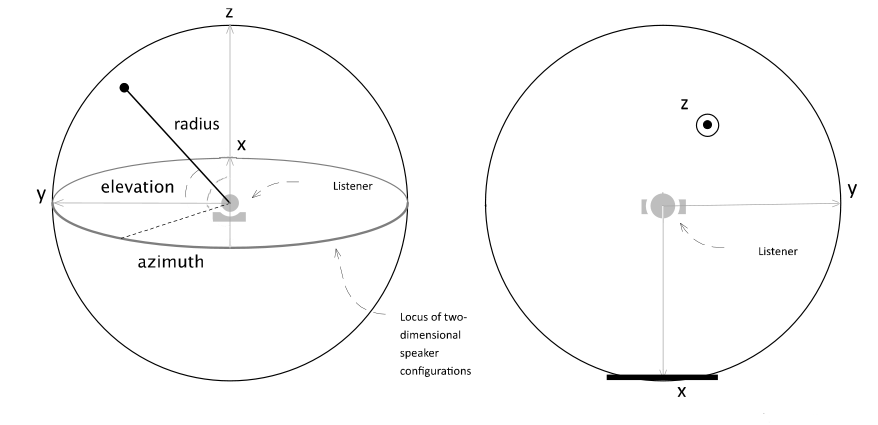
\includegraphics[scale=0.40]{figures/azimut.png}
	\caption {Coordinate spaziali}
	\label{fig:coordinate}
	\end{figure}

\item \textbf{Identificativo oggetto sonoro}: scritto come URI é un numero (int) che identifica l'oggetto sonoro, sarebbe come un indirizzo.
\item \textbf{Gain}: è un valore che indica la quantità di segnale che deve avere l'oggetto sonoro.
\item \textbf{Apertura}: scritta in gradi indicherebbe la grandezza dell'oggetto sonoro da ricreare (più l'oggetto è grande più gli altoparlanti posti marginalmente della sorgente fantasma si attivano, esempio se il valore è 180° allora si attiverebbero tutti i diffusori).
\item \textbf{Divergenza}: anch'essa indicata in gradi quantifica la grandezza che deve avere l'oggetto sonoro ma solo sul piano orizzontale, un esempio più esplicativo si ha in figura \ref{fig:apertura}

	\begin{figure}[htbp]
	\centering
	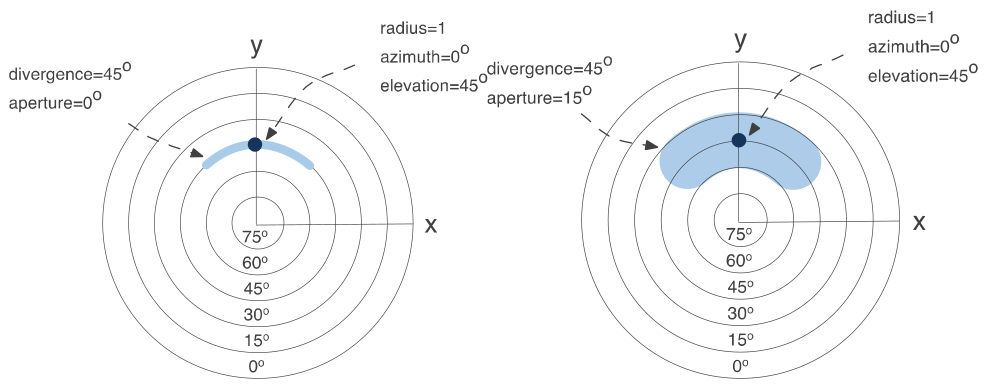
\includegraphics[scale=0.35]{figures/apertura.png}
	\caption {Parametri di apertura e divergenza}
	\label{fig:apertura}
	\end{figure}


\end{itemize}

Questi sono i principali parametri scritti nei metadati che ci servono per la spazializzazione, però è facile pensare che se l'oggetto si muove nello spazio o cambia dimensioni, il contenuto dei suoi metadati cambia anch'esso nel tempo, quindi il formato prevede di racchiude in un nuovo oggetto chiamato ''\textbf{Object-Fragment}'' tutti i metadati descritti sopra (che per tutto lo svolgimento temporale del object fragment rimarranno inalterati) con più l'aggiunta di alcuni parametri come l'\textbf{ID} (identificativo oggetto) e i sample dell'oggetto sonoro da riprodurre.

Sopra tutto poi c'è una timeline (figura \ref{fig:time}) che ha la funzione di richiamare gli object-fragment quando servono, essa è suddivisa in segmenti temporali che sono dati da $\dfrac{1}{f_c}$ dove $f_c$ è la frequenza di campionamento impostata per la totalità degli oggetti sonori e dove a ogni segmento è associato una lista di ID che richiama object-fragment da riprodurre, un esempio esplicativo è dato dallo schema \ref{fig:object}

\begin{figure}[htbp]
	\centering
	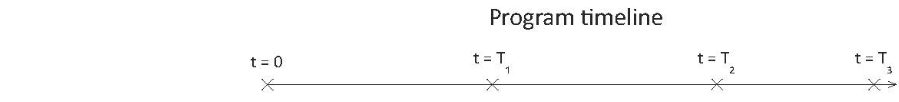
\includegraphics[scale=0.50]{figures/timeline.png}\\
	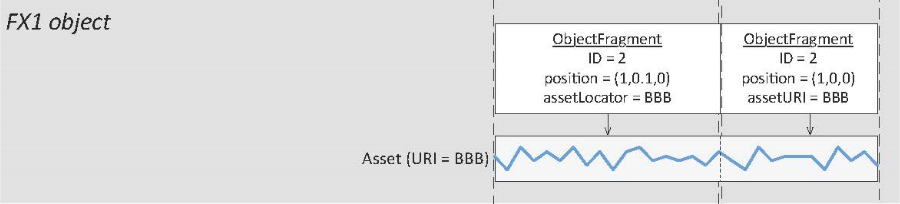
\includegraphics[scale=0.50]{figures/object1.png}\\
	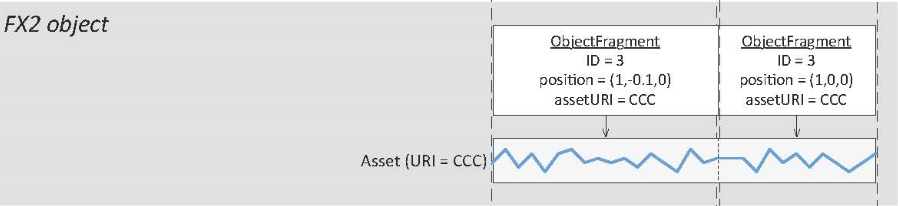
\includegraphics[scale=0.50]{figures/object2.png}\\
	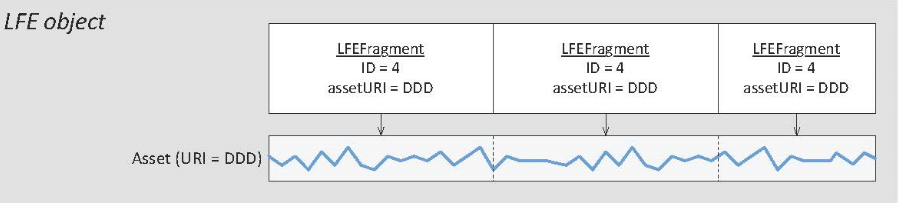
\includegraphics[scale=0.50]{figures/object3.png}
	\caption {Schema esplicativo funzionamento formato MDA}
	\label{fig:object}
	\end{figure}

\begin{figure}[htbp]
	\centering
	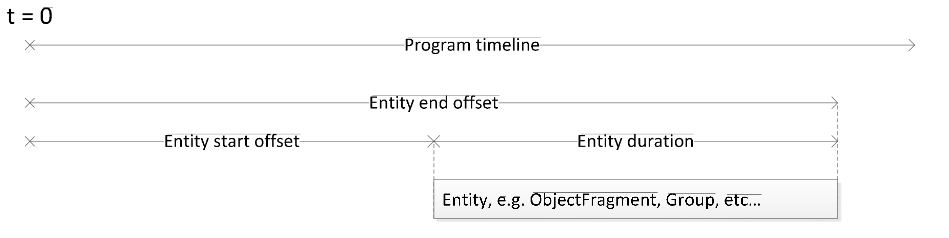
\includegraphics[scale=0.50]{figures/timeline2.png}

	\caption {Azione di richiamo di un object-fragment}
	\label{fig:time}
	\end{figure}

Da notare che è presente anche un LFE-Object in cui non è segnata la posizione, questo perché data la natura omnidirezionale delle basse frequenze non avrebbe senso collocarle spazialmente e anche perché solo il/i subwoofer sono in grado di riprodurre tali frequenze.

\subsection{Formato MDA per riproduzione audio}

Qui faccio una piccola annotazione personale, nella maggior parte dei casi quando si fa musica in studio di registrazione è abbastanza difficile che abbiamo oggetti sonori in movimento e di dimensioni che variano nel tempo, quindi si potrebbe fare una piccola modifica al formato in modo da alleggerire il successivo rendering per creare fisicamente lo spazio sonoro.

Sostanzialmente abbiamo tre tipi di oggetti sonori in musica: oggetti fermi, oggetti che ''balzano'' tra due punti spaziali ed oggetti costituiti da effetti vari (il più importante per la spazializzazione è il riverbero e per questo ci occuperemo solo di questo); tutti questi oggetti possono essere pensati come oggetti statici quindi che hanno coordinate spaziali e dimensioni fisse, in questo caso si potrebbe alleggerire il formato in quanto non avrebbe più senso parlare di object-fragment (ricordiamo che se gli attributi di spazializzazione cambiano allora si avranno diversi object-fragment, uno per ogni configurazione spaziale) in quanto per l'intera esecuzione del brano si avrebbe solo un object-fragment che fissa la posizione e la grandezza dell'oggetto, quindi si possono direttamente assegnare queste due ultime all'oggetto sonoro senza passare per ulteriori sottodivisioni.

Per quanto riguarda gli oggetti statici questo trucco calza alla perfezione, per il riverbero per esempio basterà avere come oggetto il solo contenuto del brano riverberato e assegnarli una giusta divergenza e apertura; per quanto riguarda gli oggetti ''balzanti'' (come potrebbe essere per esempio un tremolo fatto con un pan-pot in una tastiera) basterà creare in fase di post-produzione due oggetti diversi che hanno lo stesso contenuto sonoro e che differiscono soltanto per il fatto che l'intensità sonora $I'=\alpha \ \ (0\leq \alpha \leq 1)$ di un oggetto corrisponderà a una intensità $I''=(1-\alpha) I$ del secondo oggetto (dove $I$ é l'intensità totale che dovrebbe avere originariamente l'oggetto).

\section{Spazializzatore 3D}

Precedentemente abbiamo visto come è costituito il formato MDA ora non ci rimane di spiegare come produrre materiale compatibile con questo formato.

Come spiegato, nel workflow di produzione di materiale audio 3D bisognerà fermarsi prima del mixdown (sia che sia 2.0, 5.1 ecc...) e bisognerà prendere un qualche software che sia in grado di sostituire il mio mixer e sostituirlo con uno 3D, diverse aziende stanno sviluppando software di questo tipo in quanto vogliono interfacciarsi a questo formato ed in qualche modo creare un collegamento tra il loro formato proprietario e l'MDA; per esempio la Dolby ha un panner 3D per Dolby Atmos che si interfaccia con l'MDA, anche la Auro Technologies ha adottato la stessa politica o in alternativa la casa Fairlight ha creato uno spazializzatore di nome 3DAW (secondo me molto interessante) che supporta anche essa l'MDA.

Detto questo ho ricercato uno spazializzatore adatto e la mia scelta è ricaduta proprio sull'\textbf{MDA creator} proprietaria della DTS in quanto è la più intuitiva e la miglior scelta per integrazione (in quanto essa ha creato sia il panner che il formato).

Tutte le informazioni su MDA creator verranno prese dal suo manuale \cite{creator}.

Questo plugin disponibile solo per Protools è di semplice comprensione, come da manuale bisogna mettere in insert in ogni traccia questo plugin (condizione necessaria è che tutte le tracce devono avere la stessa lunghezza), poi aprendo l'interfaccia del panner bisognerà posizionare ogni oggetto nel punto in cui si desidera e con divergenza e apertura voluta (si veda il paragrafo \ref{aaa} per sapere i parametri del formato), logicamente questi parametri possono essere automatizzati per spostare e modificare l'oggetto nel tempo.

Inoltre si possono creare dei ''Bed Object'' che sarebbero oggetti i quali potranno essere direttamente codificati nel sistema di riproduzione scelto (esempio classico è la colonna sonora in 5.1 nei film) ai quali verranno sommati gli oggetti veri e propri del formato e l'LFE-Object per gli effetti a bassa frequenza.

Una volta fatto questo l'MDA creator metterà a disposizione tre scelte di output, quella che interessa a noi è la modalità di esportazione con mda file: questa scelta ci porta alla creazione dei file \textbf{.map, .mix} e \textbf{.mda} dove quest'ultimo è proprio il file contenente i metadati e gli oggetti sonori proposti in questo formato.

\begin{figure}[htbp]
	\centering
	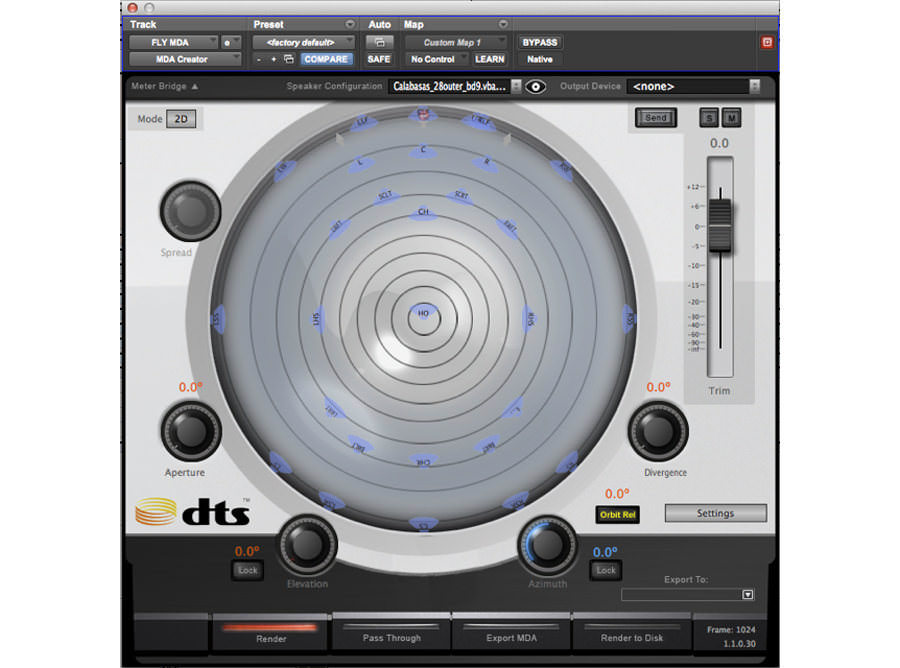
\includegraphics[scale=0.50]{figures/mdacreator.jpg}

	\caption {MDA Creator, DTS technology}
	\label{fig:mdacreator}
	\end{figure}

\chapter{Tecnica VBAP e relativa decodifica del formato MDA}

In questo capitolo parleremo invece di come da un formato MDA posso passare a una configurazione di riproduzione usuale, mediante la tecnica VBAP.

\section{Tecnica VBAP}

Il \textbf{Vector Base Amplitude Panning VBAP} è una tecnica di spazializzazione che permette di localizzare una sorgente sonora attraverso la differenza di intensità emessa tra due o più speaker, mi spiego meglio:

uno dei due parametri con cui il nostro cervello discrimina la direzione di una sorgente è la IID (si veda \cite{iid}) che indica la differenza di intensità che le nostre orecchie devono percepire per far si che si percepisca una sorgente fantasma in un punto dello spazio, quindi se riproduciamo un segnale coerente (cioè in fase fra gli altoparlanti) con minimo di due speaker e gli riproduciamo con intensità diverse, allora ci sembrerà di sentire il segnale proveniente da un punto spaziale previsto dalla IID.

Ora la cosa diventa abbastanza semplice in quanto se volgiamo ricreare una spazializzazione 2D basteranno due speaker, se invece vogliamo fare un 3D allora serviranno un minimo di 3 speaker posti a triangolo, configurazioni del genere esistono già e sono state ampiamente testate ed affinate, per tutta la documentazione riguardante il VBAP si faccia riferimento a \cite{vbap}.

E' d'obbligo affrontare un po di matematica per riuscire poi ad adattare il VBAP alle configurazioni esposte in \ref{metodi}, partiamo subito con il caso bidimensionale con 2 speaker affrontando la cosa direttamente con calcolo matriciale (all'inizio più difficile ma meglio generalizzabile per dopo).

\subsection{VBAP 2D}\label{c}
Consideriamo un sistema fatto da due speaker, definiamo ora ''arco attivo'' la porzione di circonferenza compresa tra i due speaker, ora conoscendo la posizione della nostra sorgente virtuale collocata in punto dell'arco attivo (cosa che si adatta esattamente al nostro caso) l'unica cosa che non sappiamo sono i gain $g_1$ e $g_2$ da applicare ad ogni segnale che vanno rispettivamente alle due casse per ricostruire esattamente lo spazio sonoro, quindi definendo un sistema di riferimento cartesiano $ \boldsymbol{X},\boldsymbol{Y}$ definirò come $ \boldsymbol{l_{1}}= {\left[ l_{11} \ l_{12} \right]}^T \ \  \boldsymbol{l_{2}}= {\left[ l_{21} \ l_{22} \right]}^T$ i vettori unitari che puntano verso i due altoparlanti e $\boldsymbol{p}= {\left[ p_1 \ p_2 \right]}^T$ il vettore unitario che punta verso la sorgente virtuale.

\begin{figure}[htbp]
	\centering
	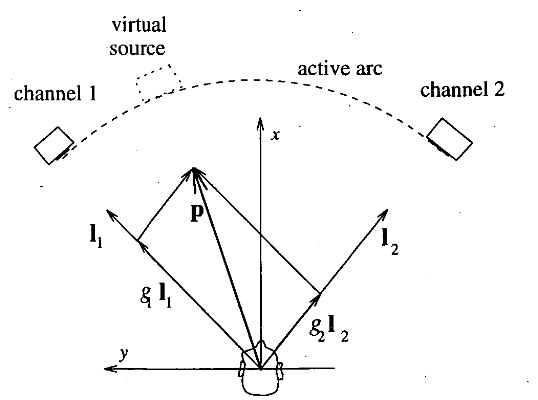
\includegraphics[scale=0.48]{figures/matrix2d.png}
	\caption {Composizione vettoriale delle sorgenti reali e virtuale}
	\label{fig:vettori2d}
	\end{figure}

Il trucco ora sta nel fatto che posso riscrivere il vettore $\boldsymbol{p}$ in funzione del vettore contenente i due gain $\boldsymbol{g}= \left[ g_1 \ g_2 \right]$ come:

\begin{equation}
\boldsymbol{p}= \boldsymbol{g} \cdot \boldsymbol{l} = \left[g_1 \ g_2 \right] \left[\boldsymbol{l_{1}} \ \boldsymbol{l_{2}} \right]^T = g_1 \boldsymbol{l_{1}} + g_2 \boldsymbol{l_{2}}
\label{eq:bbbb}
\end{equation}

In questo caso però possiamo ulteriormente compattare la scrittura in quanto:

\begin{equation}
\boldsymbol{p}=g_1 {\left[ l_{11} \ l_{12} \right]}^T + g_2 {\left[ l_{21} \ l_{22} \right]}^T= \left[ g_1 \ g_2 \right] \left[\begin{matrix}
l_{11} & l_{12}\\ l_{21} & l_{22}
\end{matrix} \right]
\label{eq:cccc}
\end{equation}

Ora trovando tutto in funzione $g$ abbiamo che:

\begin{equation}
\left[g_1 \ g_2\right] = \left[ p_1 \ p_2 \right]  {\left[\begin{matrix}
l_{11} & l_{12}\\ l_{21} & l_{22}
\end{matrix} \right]}^{-1} \ \ \Rightarrow \ \ \ \boldsymbol{g}=\boldsymbol{p}^T {\boldsymbol{L_{12}}}^{-1}
\label{eq:dddd}
\end{equation}

Logicamente assumo che la matrice $\boldsymbol{L_{12}}$ ammetta l'inversa, ora parametrizzo tutto in funzione di $\theta$ e $\theta_0$ nel modo seguente:

\[ p_1=cos(\theta),\ p_2=sen(\theta),\ l_{11}=cos(\theta_0),\ l_{12}=sen(\theta_0),\ l_{21}=cos(-\theta_0),\ l_{22}=sen(-\theta_0) \]

\begin{figure}[htbp]
	\centering
	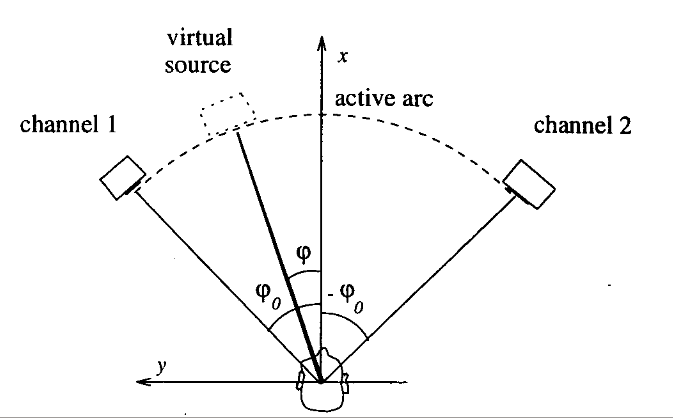
\includegraphics[scale=0.45]{figures/angoli.png}
	\caption {Angoli delle sorgenti reali e virtuale}
	\label{fig:angoli}
	\end{figure}

Fatto questo, essendo il nostro spazio ortogonale, posso calcolare direttamente i coefficienti dei due gain invertendo prima la matrice, il risultato è il seguente:

\begin{equation}\begin{split}
g_1=\dfrac{cos(\theta) sen(\theta_0) + sen (\theta) cos(\theta_0)}{2 cos(\theta_0) sen(\theta_0)}\\ \\
g_2=\dfrac{cos(\theta) sen(\theta_0) - sen (\theta) cos(\theta_0)}{2 cos(\theta_0) sen(\theta_0)}
\end{split}
\label{eq:eeee}
\end{equation}

Logicamente introduciamo un coefficiente $C$ che indica il gain complessivo (ci servirà per definire la distanza dell'oggetto) e che scalerà i nostri due gain in questo modo:

\begin{equation}
\left[g_1 \ g_2\right]_{scaled} = \dfrac{\sqrt{C} \left[ g_1 \ g_2 \right]}{\sqrt{g_1^2 + g_2^2}}
\label{eq:ffff}
\end{equation}

Sarebbe molto limitativo usare questa tecnica per ricreare una riproduzione 2.0, infatti con qualche accorgimento nulla ci vieta di poter estendere ad $n$ diffusori questa tecnica, l'unica accortezza è che il nostro procedimento dovrà ''selezionare'' solo due speaker alla quale attribuire la realizzazione della sorgente virtuale, questa scelta si basa sulla posizione dell'oggetto infatti quest'ultimo potrà essere messo solo in un arco attivo (l'intero arco giro è suddiviso in archi attivi che non si sovrappongono) quindi le due casse che delimitano questo arco saranno la coppia imputata a svolgere la riproduzione; faccio un piccolo esempio:

Consideriamo come numero $n$ arbitrario di casse consecutive $a_n$ disposte ad un angolo $\theta_{0,n}$ tali che $0°\leq \theta_{0,1},\ \theta_{0,2},\ \ldots,\ \theta_{0,n} <360°$, posizionando un qualsiasi oggetto virtuale in un qualsiasi angolo $\theta^{\prime}$ dovrà verificarsi che $\theta_{0,m}\leq \theta^{\prime} \leq \theta_{0,m+1}$ dove $m$ sta per il numero dello speaker adiacente alla sorgente virtuale ma con angolazione minore, quindi in questo caso la coppia di casse da selezionare saranno $a_m$ e $a_{m+1}$, quindi per rendere effettivo il metodo descritto nel caso di due speaker dovremo fare una piccola modifica in quanto dovremo assumere:

\begin{equation}
\theta_0 = \dfrac{\theta_{0,m+1}-\theta_{0,m}}{2} \ \ \ \ \ \theta=\theta^{\prime}-\dfrac{\theta_{0,m+1}+\theta_{0,m}}{2}
\label{phidiverso}
\end{equation}


 \begin{figure}[htbp]
	\centering
	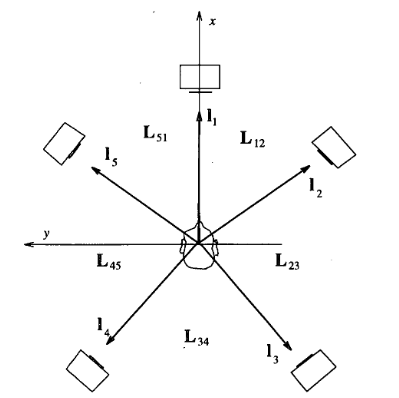
\includegraphics[scale=0.55]{figures/matrix5-1.png}
	\caption {VBAP bidimensionale con più altoparlanti}
	\label{fig:angoli5}
	\end{figure}



\subsection{VBAP 3D}

Capito qual'è il modello e l'algoritmo di implementazione del VBAP in due dimensioni estenderemo il concetto in tre dimensioni.

La più piccola configurazione di tre altoparlanti consiste nel disporli ai vertici di un triangolo equilatero come in figura \ref{fig:triangolo}, quindi ora basta prendere la formule usate sopra ed estenderle con la dimensione $\boldsymbol{Z}$ introducendo quindi l'angolo $\phi$ che indica l'elevazione dal piano orizzontale.

\begin{figure}[htbp]
	\centering
	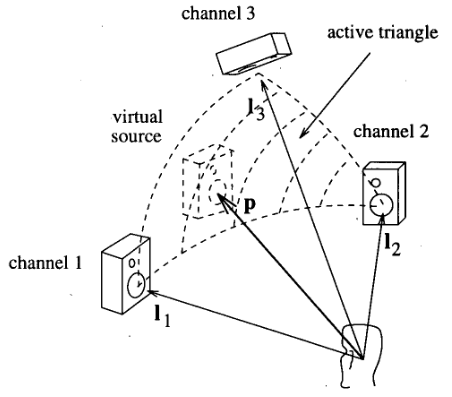
\includegraphics[scale=0.50]{figures/matrix3d.png}
	\caption {Composizione vettoriale delle sorgenti reali e virtuale in tre dimensioni}
	\label{fig:triangolo}
	\end{figure}

E' logico anche che la sorgente virtuale potrà essere collocata soltanto nella calotta\footnote{Con calotta si intende una porzione di superficie di una sfera.} delimitata dalle rette congiungenti gli altoparlanti a due a due,	 quindi esattamente come sopra se definiamo i vettori unitari che puntano alle tre casse come $ \boldsymbol{l_{1}}= {\left[ l_{11} \ l_{12} \ l_{13} \right]}^T \ \ \boldsymbol{l_{2}}= {\left[ l_{21} \ l_{22} \ l_{23} \right]}^T \ \ \boldsymbol{l_{3}}= {\left[ l_{31} \ l_{32} \ l_{33} \right]}^T$ e il vettore della sorgente virtuale $\boldsymbol{p}= {\left[ p_{1} \ p_{2} \ p_{3} \right]}^T$ risulta che:

\begin{equation}
\boldsymbol{p} = \boldsymbol{g} \cdot \boldsymbol{l} = \left[ g_1 \ g_2 \ g_3 \right] \left[ \boldsymbol{l_{1}} \ \boldsymbol{l_{2}} \ \boldsymbol{l_{3}} \right]^T
\label{gggg}
\end{equation}

Quindi ribaltando l'equazione ci rimane che:

\begin{equation}
\left[g_1 \ g_2 \ g_3 \right] = \left[ p_1 \ p_2 \ p_3 \right]  {\left[\begin{matrix}
l_{11} & l_{12} & l_{13}\\ l_{21} & l_{22} & l_{23} \\ l_{31} & l_{32} & l_{33}
\end{matrix} \right]}^{-1} \ \ \Rightarrow \ \ \ \boldsymbol{g}=\boldsymbol{p}^T {\boldsymbol{L_{123}}}^{-1}
\label{hhhh}
\end{equation}

Anche in questo caso possiamo calcolare i tre coefficienti scalati in questa maniera:

\begin{equation}
\left[g_1 \ g_2 \ g_3 \right]_{scaled} = \dfrac{\sqrt{C} \left[ g_1 \ g_2 \ g_3 \right]}{\sqrt{g_1^2 + g_2^2 + g_3^2}}
\label{iiii}
\end{equation}

In questo caso fare un esempio non è possibile in quanto il VBAP in tre dimensioni è molto legato alla geometria di implementazione e la trigonometria sulla sfera è analiticamente pesante anche se possibile, quindi si preferisce lasciare al calcolatore il compito del calcolo vettoriale senza lasciare a noi il compito di tradurre il tutto in funzioni angolari, si veda per esempio il passaggio dalla formula \ref{eq:dddd} alla formula \ref{eq:eeee}

Ora, come sopra, possiamo arrivare ad un numero $n$ di altoparlanti per coprire tutto l'angolo solido, anche qui il nostro algoritmo dovrà ''selezionare'' gli altoparlanti che saranno imputati alla riproduzione del nostro oggetto sonoro, gli stessi che delimiteranno la calotta attiva che racchiude la sorgente virtuale.

\begin{figure}[htbp]
	\centering
	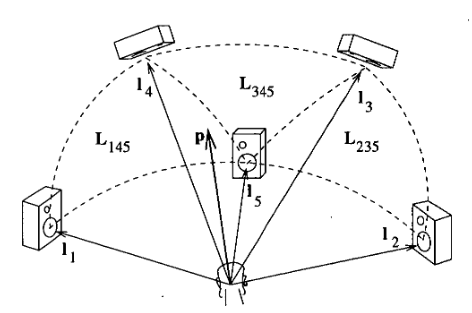
\includegraphics[scale=0.50 ]{figures/matrix3dfull.png}
	\caption {Configurazione a più altoparlanti per la tecnica VBAP in tre dimensioni}
	\label{fig:matrix3dfull}
	\end{figure}


\section{Integrazione del formatoo MDA con la tecnica VBAP}

Ricapitolando siamo arrivati al punto di sapere cos'è il formato MDA e che cos'è la tecnica di spazializzazione VBAP,
il passo successivo è riuscire ad integrare i due insieme, la cosa non è difficile ma procediamo per gradi.

N.B) nel corso di questo capitolo
ricordiamo che il formato MDA contiene oggetti sonori a cui vengono associati metadati contenenti posizione nelle tre dimensioni e grandezza, essi devono essere spacchettati e adattati in modo da essere letti dall'algoritmo del VBAP.

Un concetto fondamentale da capire è che essendo le informazioni, nei metadati, relative a uno spazio tridimensionale, esse si adatteranno benissimo a una riproduzione VBAP tridimensionale con la somma delle calotte attive coprenti l'intera superficie sferica, se il tipo di riproduzione non è questo allora bisognerà adattare i metadati in modo da poter essere congruenti all configurazione che andranno a pilotare, logicamente queste trasformazioni dovranno il più possibile lasciare inalterata la percezione spaziale a quella che è stato decisa in fase di post-produzione.

Andremo ora a vedere come integrare le due cose per alcune delle le configurazioni del capitolo \ref{metodi}

\subsection{Adattamento MDA in configurazioni tridimensionali}

Per prima cosa facciamolo per le geometrie tridimensionali, per queste non c'è bisogno di fare delle trasformazioni sulle coordinate in quante esse possono essere applicate direttamente, l'unica cosa che c'è da fare è un piccolo discorso sulle distanze e sui raggi.

Introduciamo due raggi: $r_0$ che sarebbe la lunghezza del vettore congiungente l'ascoltatore con uno degli speaker (non importa quale dato che tutti gli speaker sono posizionati sulla superficie di una sfera quindi si avranno tutti raggi uguali) e definiamo $r_1$ come la lunghezza del vettore congiungente l'ascoltatore e il più vicino degli oggetti virtuali che si vuole creare, premettendo che io posso solo riprodurre sorgenti virtuali a partire dalla superficie della sfera verso l'esterno, allora qualsiasi di questi che avranno $r_n < r_0$ non sarò in grado di riprodurli nella maniera corretta, quindi dovrò attuare una trasformazione in modo da lasciare inalterata la distanza relativa fra le sorgenti virtuali in questo modo:

\begin{equation}
\left\{\begin{matrix}
se\ \  r_1 < r_0\ \ \Rightarrow \ \ r_n^{\prime} = r_n+(r_0 - r_1) \\
\\
se\ \  r_1 \geq r_0\ \ \Rightarrow \ \ r_n^{\prime} = r_n\\
\end{matrix}\right.
\label{jjjj}
\end{equation}

fatto questo non ci rimane che intervenire sul fattore $C$ introdotto nel paragrafo \ref{c} in quanto esso contribuisce alla sensazione di lontananza, mi spiego meglio:

principalmente sono quattro i fattori che intercorrono alla corretta ricostruzione in lontananza di un oggetto, essi sono l'intensità sonora, la colorazione timbrica, il rapporto riverbero/segnale diretto e il delay temporale \footnote{La spiegazione del perché di tutti questi parametri richiederebbe molto tempo quindi diamo per buone queste assunzioni.}, l'informazione relativa agli ultimi tre parametri possono essere contenute direttamente nel segnale audio dell'oggetto sonoro, invece noi dobbiamo considerare l'intensità sonora in quanto legata alla distanza dall'oggetto all'ascoltatore e quindi al suo raggio\footnote{In realtà ogni modifica del raggio si dovrebbe ripercuote anche sugli altri tre parametri cosa che nel nostro caso non avviene essendo questi ultimi tre contenuti nell'audio dell'oggetto sonoro, siamo quindi di fronte ad un'errore ma che possiamo considerare trascurabile visto l'entità ridotta delle trasformazioni sui raggi.}.

Come detto sempre nel paragrafo \ref{c} il fattore $C$ è legato al gain complessivo dell'oggetto ma quest'ultimo posizionato sulla superficie della sfera, ora sappiamo dalla formula \ref{jjjj} che ogni oggetto è posizionato o sulla sfera o al suo esterno quindi possiamo prenderci la libertà di scalare il coefficiente $C$ in base alla distanza dell'oggetto dalla sfera in questo modo:

\begin{equation}
\boldsymbol{g_{n\ scaled}} = \dfrac{\sqrt{C_n \ f^{\prime}}\ \boldsymbol{g_n}}{\sqrt{g_1^2 +g_2^2 + g_3^2}} \ \ \ con \ \ \ \left\{\begin{matrix}
f^{\prime}= \frac{arctan\left((r_n^{\prime}-r_0)\ \dfrac{\pi}{2}\right)}{(r_n^{\prime}-r_0)\ \dfrac{\pi}{2}} & per\ r_n^{\prime}>r_0
\\
f^{\prime}=1 & per\ r_n^{\prime}=r_0
\end{matrix}\right.
\label{kkkk}
\end{equation}

In teoria l'ampiezza di un segnale sonoro dovrebbe calare con l'inverso della distanza e quindi nel nostro caso come $\frac{1}{r_n^{\prime}-r_0}$ ma facendo così avremmo dei problemi di divergenza per $r_n^{\prime}=r_0$ e valori sballati per la differenza $<1$, quindi in accordo con quanto scritto in \cite{distanza} introduco una funzione $f^{\prime}$ che approssima il più possibile la funzione originale ma che risolve totalmente i problemi nelle zone difficili (figura \ref{fig:distance}).

\begin{figure}[htbp]
	\centering
	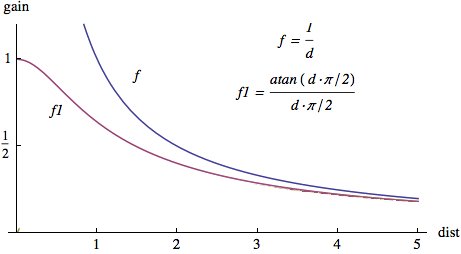
\includegraphics[scale=0.60]{figures/distance.png}
	\caption {Funzione distanza originale e funzione approssimata}
	\label{fig:distance}
	\end{figure}

Logicamente quanto detto qui sopra dovrà essere applicato in tutti casi di VBAP sia tridimensionale che non in quanto bisogna tener conto della distanza degli speaker ed è molto difficile che si abbiano tutti gli oggetti alla stessa distanza.

\subsection{Adattamento MDA in configurazioni planari}

Introduciamo ora un problema aggiuntivo: come faccio a riprodurre un programma sonoro tridimensionale in un impianto planare? questa domanda è di difficile risposta in quanto la riproduzione o meno tramite il VBAP in due dimensioni dipende dalla posizione dell'oggetto, mi spiego meglio:

Nei metadati del formato MDA sono presenti gli angoli $\theta, \phi$ e il raggio $r$ che identificano la posizione, quello che ci da informazioni sull'altezza è l'angolo (appunto detto di elevazione) $\phi$, ponendo semplicemente $\phi=0°$ sulla carta elimineremmo la dimensione verticale ma comprometteremmo anche la percezione degli oggetti originariamente posti sopra l'ascoltatore.

Per esempio, mettiamo il caso che un oggetto sia posto ad un angolo $	\theta= 90° $ e un angolo $\phi=89°$, esso praticamente si trova quasi perfettamente al disopra della nostra testa, a primo acchito verrebbe da pensare di porre semplicemente quest'ultimo a $0$ ma si avrebbe uno spostamento netto dell'oggetto alla completa sinistra dell'ascoltatore il che è incongruente con la scelta iniziale del produttore, quindi si capisce che questa strada è concettualmente sbagliata.

Contrariamente un oggetto posto a $	\theta= 90° $ con un angolo $\phi=45°$ e $r=6m$ posso tranquillamente pensarlo come proveniente solamente da sinistra visto la sua distanza dall'ascoltatore, quindi riproducibile con un VBAP in due dimensioni.

Ma vediamo ora come faccio a selezionare gli oggetti ''buoni e cattivi'' per il discorso appena fatto: per prima cosa sposto tutti gli oggetti della semisfera inferiore sopra l'ascoltatore in questo modo:

\begin{equation}
\phi_{n,top} = arctg  \left( \dfrac{\vert sen(\phi_n) \vert}{ cos(\phi_n) } \right)
\label{  b}
\end{equation}

Successivamente, tracciando la proiettante dell'oggetto nel piano orizzontale, si può vedere che gli oggetti che soddisfano l'equazione \ref{zzz} possono essere riprodotti con il VBAP tralasciando l'angolo azimutale e considerando le formule del capitolo \ref{c}

\begin{equation}
r_{n,shadow}=r_n^{\prime} cos(\phi_{n,top}) \geq r_0
\label{zzz}
\end{equation}

Tutti gli altri oggetti invece no, ma una soluzione a questi ultimi potrebbe essere di creare un ascolto immersivo per questi sfruttando tutti gli speaker del piano di ascolto e scalando il segnale da inviare a tutti questi ultimi in base alla posizione della proiettante dell'oggetto sul piano orizzontale, per esempio, nel primo caso sopra, la proiettante dell'oggetto sarebbe un punto molto vicino all'ascoltatore immediatamente alla sua sinistra, quindi i due speaker a sinistra dovrebbero riprodurre la metà più un poco di potenza sonora attribuita all'oggetto, invece gli speaker a destra la differenza per arrivare ad uno.

Un oggetto invece posto esattamente sopra l'ascoltatore potrebbe essere ricreato inviando un segnale a tutti gli $n$ speaker scalato come $\frac{1}{\sqrt{n}}$

Sicuramente in letteratura una tecnica che risolva la situazione appena citata esiste già, ma non essendo inerente alla spiegazione della tecnica VBAP verrà data già per assodata, quindi non discussa in questo testo.

\subsection{Adattamento MDA in configurazione lineare}

Per ultimo vediamo come adattare il formato alla configurazione monodimensionale, ho parlato al singolare in quanto a meno di configurazioni esoteriche si utilizzerà sempre il sistema 2.0 posto di fronte all'ascoltatore, bisogna qui stravolgere il formato in maniera pesante in quanto si devono sottrarre ben due dimensioni ma paradossalmente i passaggi da fare sono più semplici.

Come prima cosa dovrò spostare tutti gli oggetti che originariamente sono posti dietro (quindi con angoli compresi tra $90°$ e $270°$) davanti all'ascoltatore operando una trasformazione sull'angolo azimutale:

\begin{equation}
\theta_{n,front} = arctg  \left( \dfrac{sen(\theta_n)}{\vert cos(\theta_n)\vert } \right)
\label{llll}
\end{equation}

In questo modo tutti gli angoli azimutali di ogni oggetto sarà posto tra $-90° \leq \theta_{n,front} \leq +90°$

Abbiamo così ottenuto oggetti posti al massimo perfettamente ai nostri fianchi ma la configurazione 2.0 prevede al massimo una riproduzione di oggetti a $\pm 30°$ data dalla limitata ampiezza angolare $\pm \theta_0$ degli speaker, quindi dovrò rimappare gli angoli appena ottenuti in modo da essere compresi tra $0\ e \pm 30°$.

Come primo approccio ho pensato semplicemente di dividere per un fattore tre gli angoli ma accade che gli oggetti posti sullo scenario frontale vengono schiacciati troppo verso l'origine, quindi ho optato per la funzione seno (usata come peso) che schiacciasse gli oggetti posti sui lati e che lasciasse il più inalterati possibile gli angoli degli oggetti posti di fronte, in più il tutto viene ulteriormente scalato per il coseno dell'angolo di elevazione per tenere conto di quest'ultimo e della proiezione del vettore sul piano orizzontale, in questo modo:

\begin{equation}
\theta_{n, remapped}= \theta_0 \cos(\phi) \ sen (\theta_{n,front}) = \theta_0 \cos(\phi)\ sen \left( arctg  \left( \dfrac{sen(\theta_n)}{\vert cos(\theta_n)\vert } \right)\right)
\label{mmmm}
\end{equation}





\subsection{Esempio di integrazione con sistemi quadrifonico, 5.1 e 2.0}

Per tutti gli esempi che farò vorrò riprodurre tre oggetti con seguenti coordinate sferiche per far vedere ogni caso:\\

\begin{tabular}{|c|c|c|c|c|}
\hline
oggetto 1 & $\theta_1=15°$ & $\phi_1=0°$ & $r_1=1,5m$ & $C_1=1,3$ \\
\hline
oggetto 2 & $\theta_2=275°$ & $\phi_2=0°$ & $r_2=2,5m$ & $C_2=1,6$ \\
\hline
oggetto 3 & $\theta_3=160°$ & $\phi_3=45°$ & $r_3=3,0m$ & $C_1=0,8$ \\
\hline

\end{tabular} \\ \\

N.B) ai fini dei calcoli conviene pensare $\theta_2=275°$ come $\theta_2=-85°$.\\

Cominciamo con la quadrifonia, una possibile configurazione potrebbe essere questa:\\

\begin{tabular}{|c|c|c|}
\hline
speaker 1 & $\theta_{0,1}=45°$ & $r_0=2m$\\
\hline
speaker 2 & $\theta_{0,2}=135°$ & $r_0=2m$\\
\hline
speaker 3 & $\theta_{0,3}=-135°$ & $r_0=2m$\\
\hline
speaker 4 & $\theta_{0,4}=-45°$ & $r_0=2m$\\
\hline
\end{tabular} \\
\\

Come prima cosa applichiamo la formula \ref{jjjj} in modo da scalare i raggi degli oggetti e rendergli:

\[r_1^{\prime}=2m \ \  r_2^{\prime}=3m \ \ r_3^{\prime}=3,5m  \]

Ora è facile trovare i gain e i gain scalati del primo e del secondo oggetto in quanto il primo è riprodotto dagli speaker 4 e 1 invece il secondo dagli speaker 3 e 4 in questo modo:

per entrambi gli oggetti, prima applico la formula \ref{phidiverso} in modo da trovare i nuovi angoli da mettere nella formula \ref{eq:eeee} poi considerando i coefficienti $C_n$ e i raggi $r_n^{\prime}$ ricavo dalla formula \ref{kkkk} i gain scalati per entrambi gli oggetti che in questo caso saranno:

\begin{equation}
\begin{matrix}
g_{(1,obj\ 1)} = 0,87 & g_{(1,obj\ 1)scaled} = 0,861\\
g_{(4,obj\ 1)} = 0,50 & g_{(4,obj\ 1)scaled} = 0,733\\
g_{(4,obj\ 2)} = 0,76 & g_{(4,obj\ 2)scaled} = 0,779\\
g_{(3,obj\ 2)} = 0,64 & g_{(3,obj\ 2)scaled} = 0,651\\
\end{matrix}
\label{gscalatiesempio1}
\end{equation}
\\

Passiamo ora all'adattamento alla configurazione 5.1

Una possibile configurazione di impianto 5.1 potrebbe essere la seguente:

\begin{tabular}{|c|c|c|}
\hline
speaker 1 & $\theta_{0,1}=0°$ & $r_0=2m$\\
\hline
speaker 2 & $\theta_{0,2}=30°$ & $r_0=2m$\\
\hline
speaker 3 & $\theta_{0,3}=110°$ & $r_0=2m$\\
\hline
speaker 4 & $\theta_{0,4}=-110°$ & $r_0=2m$\\
\hline
speaker 5 & $\theta_{0,4}=-30°$ & $r_0=2m$\\
\hline
\end{tabular} \\
\\

Non ci rimane che operare nella stessa maniera utilizzata per la quadrifonia esposta appena sopra (infatti si applicheranno esattamente le stesse formule con l'unica differenza di avere dei $\theta_{0,n}$ visibilmente diversi), ricavo così i gain e i gain scalati degli speaker 2 e 1 (imputati alla riproduzione del primo oggetto) e 5 e 4 (imputati alla riproduzione del secondo):

\begin{equation}
\begin{matrix}
g_{(2,obj\ 1)} = 0,52 & g_{(2,obj\ 1)scaled} = 0,806\\
g_{(1,obj\ 1)} = 0,52 & g_{(1,obj\ 1)scaled} = 0,806\\
g_{(5,obj\ 2)} = 0,43 & g_{(5,obj\ 2)scaled} = 0,465\\
g_{(4,obj\ 2)} = 0,83 & g_{(4,obj\ 2)scaled} = 0,898  \\

\end{matrix}
\label{gscalatiesempio2}
\end{equation} \\


Volutamente, per entrambe le configurazioni, ho tralasciato la riproduzione del terzo oggetto in modo da riprenderlo qui, infatti per prima bisogna vedere se esso verifica l'equazione \ref{zzz} cosa che avviene, poi si provvede a calcolare normalmente i gain e i gain scalati della oggetto rispettivamente nella configurazione quadrifonica e 5.1 dando i seguenti risultati:

\begin{equation}
\begin{matrix}
g_{(3,obj\ 3)} = 0,42 & g_{(3,obj\ 3)scaled} = 0,266\\
g_{(2,obj\ 3)} = 0,90 & g_{(2,obj\ 3)scaled} = 0,571\\
\\
g_{(4,obj\ 3)} = 1,19 & g_{(4,obj\ 3)scaled} = 0,383\\
g_{(3,obj\ 3)} = 1,55 & g_{(3,obj\ 3)scaled} = 0,499\\

\end{matrix}
\label{gscalatiesempiooggetto3}
\end{equation} \\



Per ultimo esempio vediamo il risultato dell'adattamento alla configurazione 2.0.

Una configurazione possibile potrebbe essere la seguente:

\begin{tabular}{|c|c|c|}
\hline
speaker 1 & $\theta_{0,1}=30°$ & $r_0=2m$\\
\hline
speaker 2 & $\theta_{0,2}=-30°$ & $r_0=2m$\\
\hline
\end{tabular} \\
\\

Applicando rispettivamente la formula \ref{llll} e la formula \ref{mmmm} ottengo i seguenti risultati:


\begin{tabular}{|c|c|}
\hline
$\theta_{1,front} = 15°$     & $\theta_{1,remapped} =  8°  $   \\
\hline
$\theta_{2,front} = -85°$     & $\theta_{2,remapped} = -29° $     \\
\hline
$\theta_{3,front} = 20°$    & $ \theta_{3,remapped} =  7° $    \\
\hline
\end{tabular} \\
\\

Ora non ci rimane da trovare i gain degli oggetti tramite la formula \ref{eq:eeee} e i gain scalati con la \ref{kkkk}

\begin{equation}
\begin{matrix}
g_{(1,obj\ 1)} = 0,71 & g_{(1,obj\ 1)scaled} = 0,975\\
g_{(2,obj\ 1)} = 0,43 & g_{(2,obj\ 1)scaled} = 0,590\\
g_{(1,obj\ 2)} = 0,02 & g_{(1,obj\ 2)scaled} = 0,021\\
g_{(2,obj\ 2)} = 0,99 & g_{(2,obj\ 2)scaled} = 1,011\\
g_{(1,obj\ 3)} = 0,69 & g_{(1,obj\ 3)scaled} = 0,524\\
g_{(2,obj\ 3)} = 0,46 & g_{(2,obj\ 3)scaled} = 0,349\\
\end{matrix}
\label{gscalatiesempio3}
\end{equation}










\chapter*{Conclusioni}

Sviluppando questa tesi quindi, è stata affrontata bene la filosofia di implementazione dell'audio a oggetti e si è visto la sua utilità e versatilità nel campo del audio-video e del solo audio implementandola nelle più conosciute configurazioni di riproduzione.

Questo sviluppo però getta solo le basi per un suo impiego, si dovrò approfondire di più l'argomento per raffinarlo e renderlo anch'esso uno standard fruibile a tutti.

Logicamente in questa scrittura ho affrontato solo alcuni adattamenti del formato MDA in alcune configurazioni attraverso il VBAP, ma per la sua malleabilità l'audio ad oggetti si presta benissimo anche all'implementazione con la tecnica ambisonic, binaurale (nonché ambiophonic) e soprattutto con la tecnica WFS che potrà magari in futuro prendere piede nell'audio consumer, ma tutte queste sono storie in un'altra lettura.



\addcontentsline{toc}{chapter}{Conclusioni}

\begin{thebibliography}{}

\bibitem{5.1} \textit{https://www.itu.int/dms\_pubrec/itu-r/rec/bs/R-REC-BS.775-3-201208-I!!PDF-E.pdf}
\bibitem{quadraphonic} \textit{http://www.dith.it/listing/master/dispense\%20Schiavoni/CSE10-08.pdf}
\bibitem{digital} \textit{https://it.wikipedia.org/wiki/Dolby\_Digital}
\bibitem{surround} \textit{http://www.dith.it/listing/master/dispense\%20Schiavoni/CSE10-08.pdf}
\bibitem{atmos} \textit{https://www.dolby.com/us/en/technologies/dolby-atmos/dolby-atmos-next-generation-audio-for-cinema-white-paper.pdf}
\bibitem{mda}\textit{http://www.etsi.org/deliver/etsi\_ts/103200\_103299/103223/01.01.01\_60/ts\_103223v010101p.pdf}
\bibitem{creator}\textit{//digitalcommons.calpoly.edu/cgi/viewcontent.cgi?article=1049}\&\textit{context=laessp}
\bibitem{iid} \textit{https://en.wikipedia.org/wiki/Sound\_localization\#ITD\_and\_IID}
\bibitem{vbap} \textit{http://lib.tkk.fi/Diss/2001/isbn9512255324/article1.pdf}
\bibitem{distanza} \textit{http://write.flossmanuals.net/csound/b-panning-and-spatialization/}
\end{thebibliography}

\addcontentsline{toc} {chapter}{Bibliografia}


\end{document}
